% % % % mainfile: ../../../../master.tex
% \subsection{C++ Statements}
% \label{task:20231206_cpp}

% An expression becomes an expression statement when it is followed by a semicolon. Expression statements cause the expression to be evaluated and its result discarded:
% \begin{lstlisting}[language=C++]
% ival + 5;       // rather useless expression statement 
% cout << ival;   // useful expression statement
% \end{lstlisting}

% Null statement is a single semicolon, and is legal anywhere a statement is expected:
% \begin{lstlisting}[language=C++]
% ;                   // null statement
% ival = v1 + v2;;    // ok: second semicolon is a superfluous null statement

% // disaster: extra semicolon: loop body is this null statement 
% while (iter != svec.end()) ; // the while body is the empty statement 
%     ++iter; // increment is not part of the loop
% \end{lstlisting}

% A compound statement, usually referred to as a block, is a sequence of statements and declarations surrounded by a pair of curly braces. Names introduced inside a block are accessible only in that block and in blocks nested inside that block.

% \subsubsection{Conditional Statements}

% An \texttt{if} statement conditionally executes another statement based on whether a specified condition is true:
% \begin{lstlisting}[language=C++]
% if (condition)
%     statement
% else
%     statement2
% \end{lstlisting}

% We use a block to enclose multiple statements:
% \begin{lstlisting}[language=C++]
% // if failing grade, no need to check for a plus or minus 
% if (grade < 60) 
%     lettergrade = scores[0]; 
% else { 
%     lettergrade = scores[(grade - 50)/10]; // fetch the letter grade 
%     if (grade != 100) // add plus or minus only if not already an A++ 
%         if (grade % 10 > 7) lettergrade += '+'; // grades ending in 8 or 9 get a + 
%             else if (grade % 10 < 3) 
%             lettergrade += '-'; // grades ending in 0, 1,or 2 get a 
% }
% \end{lstlisting}
% It is a common mistake to forget the curly braces when multiple statements must be executed as a block.

% Danglging \texttt{else} is resolved by specifying that each \texttt{else} matched with the closest preceding unmatched \texttt{if}:
% \begin{lstlisting}[language=C++]
% // WRONG: execution does NOT match indentation; the else goes with the inner if 
% if (grade % 10 >= 3) 
%     if (grade % 10 > 7) 
%         lettergrade += '+'; // grades ending in 8 or 9 get a + 
% else 
%     lettergrade += '-'; // grades ending in 3, 4, 5, 6, or 7 get a minus!

% // add a plus for grades that end in 8 or 9 and a minus for those ending in 0, 1, or 2 
% if (grade % 10 >= 3) { 
%     if (grade % 10 > 7) 
%         lettergrade += '+'; // grades ending in 8 or 9 get a + 
% } else // curlies force the elseto go with the outer if 
%     lettergrade += '-'; // grades ending in 0, 1, or 2 will get a minus
% \end{lstlisting}
% We can make the else part of the outer if by enclosing the inner if in a block.

% \subsubsection{Iterative Statements}

% The syntactic form of the \texttt{for} statement is:
% \begin{lstlisting}[language=C++]
% // for (initializer; condition; expression) 
% //     statement

% // process characters in s until we run out of characters or we hit a whitespace 
% for (decltype(s.size()) index = 0; 
%         index != s.size() && !isspace(s[index]); ++index)     
%     s[index] = toupper(s[index]); // capitalize the current character
% \end{lstlisting}

% The order of evaluation of \texttt{for} loop:
% \begin{enumerate}
% \item \textit{init-statement} is executed once at the start of the loop. 
% \item Next, \textit{condition} is evaluated.
% \item If the condition is \texttt{true}, the \texttt{for} body executes. 
% \item Finally, \textit{expression} is evaluated. 
% \end{enumerate}

% \textit{init-statement} can define several objects in a single declaration statement:
% \begin{lstlisting}[language=C++]
% // remember the size of v and stop when we get to the original last element 
% for (decltype(v.size()) i = 0, sz = v.size(); i != sz; ++i) 
%     v.push_back(v[i]);
% \end{lstlisting}

% A \texttt{for} header can omit any (or all) of \textit{init-statement}, \textit{condition}, or \textit{expression}, by replacing them with null statements:
% \begin{lstlisting}[language=C++]
% auto beg = v.begin(); 
% for ( /* null */; beg != v.end() && *beg >= 0; ++beg) 
%     ;// no work to do

% // Omitting condition is equivalent to writing true as the condition
% for (int i = 0; /* no condition */ ; ++i) { 
%     // process i; code inside the loop must stop the iteration! 
% }

% // If we omit expression for the for header, either the condition or the body must do something to advance the iteration
% vector<int> v; 
% for (int i; cin >> i; /* no expression */) 
%     v.push_back(i);
% \end{lstlisting}

% The syntactic form of range \texttt{for} statement to iterate through elements of a container or other sequence:
% \begin{lstlisting}[language=C++]
% // for (declaration: expression)
% //     statement
% \end{lstlisting}
% \textit{expression} must represent a sequence such as braced initializer list, array or object of type such as \texttt{vector} or \texttt{string} that has \texttt{begin} and \texttt{end} members that return iterators. \textit{declaration} defines a variable. It must be possible to convert each element of the sequence to the variable's type. The easiest way to make sure the types match is to use the \texttt{auto} type specifier. 

% \subsubsection{Jump Statements}



% % The relational operators take operands of arithmetic or pointer type; the logical operators take operands of any type that can be converted to \texttt{bool}. The operands to those operators are rvalues and the result is an rvalue.

% % \begin{longtable}{p{.15\linewidth}p{.1\linewidth}p{.25\linewidth}p{.25\linewidth}} 
% % \toprule
% % Associativity & Operator & Function & Use \\
% % \midrule
% % \endhead

% % Right
% % &\texttt{!}
% % &logical \texttt{NOT}
% % &\texttt{!expr}
% % \\

% % Left
% % &\texttt{<}
% % &less than
% % &\texttt{expr < expr}
% % \\

% % Left
% % &\texttt{<=}
% % &less than or equal
% % &\texttt{expr <= expr}
% % \\

% % Left
% % &\texttt{>}
% % &greater than
% % &\texttt{expr > expr}
% % \\

% % Left
% % &\texttt{>=}
% % &greater than or equal
% % &\texttt{expr >= expr}
% % \\

% % \midrule

% % Left
% % &\texttt{==}
% % &equality
% % &\texttt{expr == expr}
% % \\

% % Left
% % &\texttt{!=}
% % &inequality
% % &\texttt{expr != expr}
% % \\

% % \midrule

% % Left
% % &\texttt{\&\&}
% % &logical \texttt{AND}
% % &\texttt{expr \&\& expr}
% % \\

% % \midrule

% % Left
% % &\texttt{||}
% % &logical \texttt{OR}
% % &\texttt{expr || expr}
% % \\

% % \midrule
% % \caption{Logical and Relational Operators} 
% % \label{tab:logicalrelationaloperators}
% % \end{longtable}

% % Because relational operators return \texttt{bool}s, the result of chaining these operators together is likely to be surprising:
% % \begin{lstlisting}[language=C++]
% % // oops! this condition compares k to the bool result of i<j 
% % if(i<j<k) // true if k is greater than 1!
% % \end{lstlisting}

% % The compiler converts \texttt{val} to \texttt{bool}:
% % \begin{lstlisting}[language=C++]
% % if (val) { /* ... */} // true if val is any nonzero value 
% % if (!val) { /* ... */}// true if val is zero
% % if (val == true) { /* ... */}// trueonly if valis equal to 1!
% % if (val == 1) { /* ... */}
% % \end{lstlisting}
% % If \texttt{val} is not \texttt{bool}, then \texttt{true} is converted to the type of \texttt{val} before the \texttt{==} operator is applied. 

% % \subsubsection{Assignment Operators}

% % The left-hand operand of an assignment operator must be a modifiable lvalue. For example, given:
% % \begin{lstlisting}[language=C++]
% % int i = 0, j = 0, k = 0;    // initializations, not assignment 
% % const int ci = i;           // initialization, not assignment
% % 1024 = k;                   // error: literals are rvalues 
% % i + j = k;                      // error: arithmetic expressions are rvalues 
% % ci = k;                     // error: ci is a const(nonmodifiable) lvalue
% % k = 0;                      // result: type int, value 0 
% % k = 3.14159;                // result: type int, value 3
% % k = {3.14};                 // error: narrowing conversion 
% % vector<int> vi;             // initially empty 
% % vi = {0,1,2,3,4,5,6,7,8,9}; // vi now has ten elements, values 0 through 9
% % \end{lstlisting}

% % Unlike the other binary operators, assignment is right associative. The right-most assignment, \texttt{jval = 0}, is the right-hand operand of the left-most assignment operator:
% % \begin{lstlisting}[language=C++]
% % int ival, jval; 
% % ival = jval = 0; // ok: each assigned 0
% % int ival, *pval; // ival is an int; pval is a pointer to int 
% % ival = pval = 0; // error: cannot assign the value of a pointer to an int 
% % string s1, s2; 
% % s1 = s2 = "OK"; // string literal "OK"converted to string
% % \end{lstlisting}
% % Each object in a multiple assignment must have the same type as its right-hand neighbor or a type to which that neighbor can be converted.

% % Assignment often occur in conditions. Because assignment has relatively low precedence, we usually must parenthesize the assignment for the condition to work properly:
% % \begin{lstlisting}[language=C++]
% % // a verbose and therefore more error-prone way to write this loop 
% % int i = get_value(); // get the first value 
% % while (i != 42) { 
% %     // do something . . . 
% %     i = get_value(); 
% %     // get remaining values 

% % }

% % int i; 
% % // a better way to write our loop---what the condition does is now clearer 
% % while ((i = get_value()) != 42) { 
% %     // do something . . . 
% % }
% % \end{lstlisting}

% % \subsubsection{Assignment Operators}

% % The dot and arrow operators provide for member access. The dot operator fetches a member from an object from an object of class type; arrow is defined so that \textit{ptr->mem}  is a synonym for \textit{(*ptr).mem)}:
% % \begin{lstlisting}[language=C++]
% % string s1 = "a string", *p = &s1; 
% % auto n = s1.size(); // run the sizemember of the strings1 
% % n = p->size();      // equivalent to (*p).size()
% % n=(*p).size();      // run size on the object to which p points 

% % // run the size member of p, then dereference the result! 
% % *p.size(); // error: p is a pointer and has no member named size
% % \end{lstlisting}
% % Because dereference has a lower precedence than dot, we must parenthesize the dereference subexpression.

% % \subsubsection{Conditional Operator}

% % The conditional (the \texttt{?:} operator) lets us embed simple if-else logic inside an expression:
% % \begin{lstlisting}[language=C++]
% % // cond ? expr1: expr2;
% % string final grade = (grade < 60) ? "fail": "pass";
% % \end{lstlisting}
% % where \texttt{expr1} and \texttt{expr2} are expressions of the same type.

% % An incompletely parenthesized conditional operator in an output expression can have surprising results:
% % \begin{lstlisting}[language=C++]
% % cout << ((grade < 60) ? "fail" : "pass"); // prints pass or fail 
% % cout << (grade < 60) ? "fail" : "pass"; // prints 1 or 0! 
% % cout << grade < 60 ? "fail" : "pass"; // error: compares cout to 60
% % \end{lstlisting}
% % The second expression uses the comparison between \texttt{grade} and \texttt{60} as the operand to the \texttt{<<} operator. 

% % \subsubsection{Bitwise Operator}

% % Because there are no guarantees for how the sign bit is handled, it is strongly recommended to use \texttt{unsigned} types with the bitwise operators.

% % \begin{longtable}{p{.2\linewidth}p{.3\linewidth}p{.3\linewidth}} 
% % \toprule
% % Operator & Function & Use \\
% % \midrule
% % \endhead

% % \texttt{~}
% % &bitwise \texttt{NOT}
% % &\texttt{~expr}
% % \\

% % \midrule

% % \texttt{<<}
% % &left shift
% % &\texttt{expr1 << expr2}
% % \\
% % \texttt{>>}
% % &right shift
% % &\texttt{expr1 >> expr2}
% % \\
% % \midrule

% % \texttt{\&}
% % &bitwise \texttt{AND}
% % &\texttt{expr1 \& expr2}
% % \\
% % \midrule

% % \texttt{\^}
% % &bitwise \texttt{XOR}
% % &\texttt{expr1 \^ expr2}
% % \\
% % \midrule

% % \texttt{|}
% % &bitwise \texttt{OR}
% % &\texttt{expr1 | expr2}
% % \\

% % \midrule
% % \caption{Bitwise Operators} 
% % \label{tab:bitwiseoperators}
% % \end{longtable}

% % The built-in menaing of the shift operators is to perform a bitwise shift on their operands. They yield a value that is a copy of the left-hand operand with the bits shifted as directed by the right-hand operand. The right-hand operand must not be negative and must be a value that is strictly less than the number of bits in the result. Otherwise, the operation is undefined. The bits are shifted left (\texttt{<<}) or right (\texttt{>>}). Bits that are shifted off the end are discarded:
% % \begin{figure}[H]
% %     \centering
% %     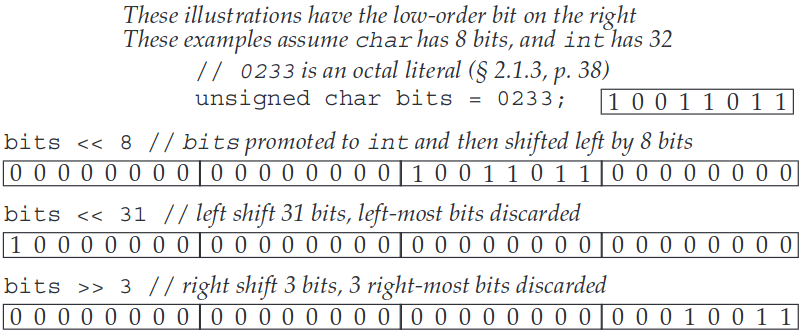
\includegraphics[width=.95\linewidth]{entries/2023/12/05/bitshift.png}
% %     \caption{Bitwise Shift Operation}
% %     \label{fig:bitshift}
% % \end{figure}

% % Shift operators have midlevel precedence (lower than the arithmetic operators but higher than the relational, assignment, and conditional operators):
% % \begin{lstlisting}[language=C++]
% % cout << 42 + 10; // ok: + has higher precedence, so the sum is printed 
% % cout << (10 < 42); // ok: parentheses force intended grouping; prints 1  
% % cout << 10 < 42; // error: attempt to compare cout to 42!
% % \end{lstlisting}

% % The bitwise NOT operator generates a new value with the bits of its operand inverted:
% % \begin{figure}[H]
% %     \centering
% %     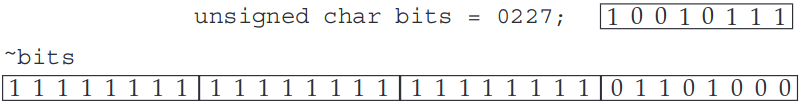
\includegraphics[width=.85\linewidth]{entries/2023/12/05/bitnot.png}
% %     \caption{Bitwise NOT Operation}
% %     \label{fig:bitnot}
% % \end{figure}

% % The AND, OR, and XOR operators generate new values with the bit pattern composed from its two operands:
% % \begin{figure}[H]
% %     \centering
% %     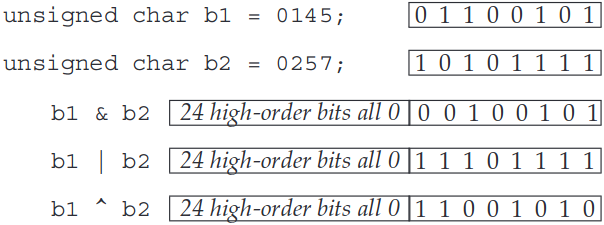
\includegraphics[width=.75\linewidth]{entries/2023/12/05/bitoth.png}
% %     \caption{Bitwise AND, OR, and XOR Operation}
% %     \label{fig:bitoth}
% % \end{figure}

% % \subsubsection{\texttt{sizeof} Operator}

% % The \texttt{sizeof} operator returns the size, in bytes, of an expression or a type name. The operator is right associative. The result of \texttt{sizeof} is a constant expression of type \path{size_t}. The operator takes one of two forms:
% % \begin{lstlisting}[language=C++]
% % sizeof(type)
% % sizeof expr
% % \end{lstlisting}

% % The \texttt{sizeof} operator is unusual in that it does not evaluate its operand:
% % \begin{lstlisting}[language=C++]
% % Sales_data data, *p; 
% % sizeof(Sales_data); // size required to hold an object of type Sales_data 
% % sizeof data; // size of data's type, i.e., sizeof(Sales_data) 
% % sizeof p; // size of a pointer 
% % sizeof *p; // size of the type to which p points, i.e., sizeof(Sales_data) 
% % sizeof data.revenue; // size of the type of Sales_data's revenue member 
% % sizeof Sales_data::revenue; // alternative way to get the size of revenue
% % \end{lstlisting}
% % Dereferencing an invalid pointer as the operand to \texttt{sizeof} is safe because the pointer is not actually used, because \texttt{sizeof} does not need to dereference the pointer to know what type it will return.

% % The result of applying \texttt{sizeof} depends in part on the type involved:
% % \begin{itemize}
% %     \item \texttt{sizeof char} or an expression of type \texttt{char} is guaranteed to be 1.
% %     \item \texttt{sizeof} a reference type returns the size of an object of the referenced type.
% %     \item \texttt{sizeof} a pointer returns the size needed to hold a pointer.
% %     \item \texttt{sizeof} a dereferenced pointer returns the size of an object of the type to which the pointer points; the pointer need not be valid.
% %     \item \texttt{sizeof} an array is the size of the entire array. It is equivalent to taking the \texttt{sizeof} the element type times the number of elements in the array. Note that \texttt{sizeof} does not convert the array to a pointer.
% %     \item \texttt{sizeof} a \texttt{string} or a \texttt{vector} returns only the size of the fixed part of these types; it does not return the size used by the object's elements.
% % \end{itemize}
% % Because \texttt{sizeof} returns the size of the entire array, we can determine the number of elements in an array by dividing the array size by the element size.

% % \subsubsection{Comma Operator}

% % The comma operator takes two operands, which it evaluates from left to right. Like the logical AND and logical OR and the conditional operator guarantees the order in which its operands are evaulated. Most common use for the comma operator is in a \texttt{for} loop:
% % \begin{lstlisting}[language=C++]
% % vector<int>::size_type cnt = ivec.size(); 
% % // assign values from size...1 to the elements in ivec 
% % for(vector<int>::size_type ix = 0; 
% %         ix != ivec.size(); ++ix, --cnt) 
% %     ivec[ix] = cnt;
% % \end{lstlisting}
% % The left-hand expression is evaluated and its result is discarded. The result of a comma expression is the value of its right-hand expression. The result is an lvalue if the right-hand operand is an lvalue.

% % \subsubsection{Type Conversions}

% % Implicit conversions are carried out automatically without programmer intervention, and are defined to preserve precision, if possible. 
% % \begin{itemize}
% %     \item In most expressions, values of integral types smaller than \texttt{int} are first promoted to an appropriate larger integral type.
% %     \item In conditions, non\texttt{bool} expressions are converted to \texttt{bool}.
% %     \item In initializations, the initializer is converted to the type of the variable; in assignments, the right-hand operand is converted to the type of the left-hand.
% %     \item In arithmetic and relational expressions with operands of mixed types, the types are converted to a common type.
% % \end{itemize}
% % Conversions also happen during function calls.

% % Arithmetic conversions:
% % \begin{lstlisting}[language=C++]
% % bool flag;      char cval; 
% % short sval;     unsigned short usval; 
% % int ival;       unsigned int uival; 
% % long lval;      unsigned long ulval; 
% % float fval;     double dval; 

% % 3.14159L + 'a'; // 'a' promoted to int, then that intconverted to long double 
% % dval + ival; // ival converted to double 
% % dval + fval; // fval converted to double 
% % ival = dval; // dval converted (by truncation) to int 
% % flag = dval; // if dval is 0,then flag is false, otherwise true 
% % cval + fval; // cval promoted to int, then that int converted to float 
% % sval + cval; // sval and cval promoted to int
% % cval + lval; // cval converted to long 
% % ival + ulval; // ival converted to unsigned long 
% % usval + ival; // promotion depends on the size of unsigned short and int 
% % uival + lval; // conversion depends on the size of unsigned int and long
% % \end{lstlisting}

% % Array to pointer conversion:
% % \begin{lstlisting}[language=C++]
% % int ia[10]; // array of ten ints 
% % int* ip = ia; // convert ia to a pointer to the first element
% % \end{lstlisting}
% % This conversion is not performed when an array is used with \texttt{decltype} or as the operand of the address-of(\texttt{\&}), \texttt{sizeof}, or \texttt{typeid} operators. The conversion is also omitted when we initialize a reference to an array. A similar pointer conversion happens when we use a function type in an expression.

% % A constant integral value of \texttt{0} and the literal \texttt{nullptr} can be converted to any pointer type; a pointer to any non\texttt{const} type can be converted to \texttt{void*}, and a pointer to any type can be converted to a \texttt{const void*}

% % There is an automatic conversion from arithmetic or pointer types to \texttt{bool}. If the pointer or arithmetic value is zero, the conversion yields \texttt{false}; any other yields \texttt{true}:
% % \begin{lstlisting}[language=C++]
% % char *cp = get_string(); 
% % if (cp) /* ... *///     trueif the pointer cp is not zero 
% % while (*cp) /* ... */// trueif *cpis not the null character
% % \end{lstlisting}

% % We can convert a pointer to a non\texttt{const} type to a pointer to the corresponding \texttt{const} type, and similarly for references. That is, if \texttt{T} is a type, we can convert a pointer or a  reference to \texttt{T} into a pointer or a reference to \texttt{const T}:
% % \begin{lstlisting}[language=C++]
% % int i; 
% % const int &j = i; // convert a non const to a reference to const int 
% % const int *p = &i; // convert address of a non const to the address of a const 
% % int &r = j, *q = p; // error: conversion from const to nonconst not allowed
% % \end{lstlisting}
% % The reverse conversion - removing a low-level \texttt{const} - does not exist.
